%!TEX TS-program = XeLaTeX
%!TEX TS-program = XeLaTeX
\documentclass[11pt]{article}

\usepackage{amssymb}
\usepackage{amsthm}
\usepackage{amsmath}
\usepackage{mathtools}

\usepackage{fancyhdr}
\usepackage{graphicx}
\usepackage[top=3cm, left=2cm, right=2cm, headheight = 90pt]{geometry}
\usepackage{xltxtra}
\usepackage[font=small,labelfont=bf]{caption}

\usepackage{multicol}

\renewcommand{\theenumi}{\alph{enumi}}


\def\leq{\leqslant}
\def\geq{\geqslant}
\def\N{\mathbb N}
\def\R{\mathbb R}
\def\Z{\mathbb Z}
\DeclarePairedDelimiter\set\{\}

\def\prob{}

\theoremstyle{definition}
\newtheorem{problem}{\prob}


\pagestyle{fancy}

%!TEX TS-program = XeLaTeX

\fancyfoot[CE,CO]{}  % this is to remove page numbers (as you might want for single page docs)

%!TEX TS-program = XeLaTeX
\renewcommand{\figurename}{Attēls}


\fancyhead[C]{{\Large\bf Grafi 1 - Uzdevumi}\\ \date}

\begin{document}

\noindent 
%\emph{\notes}

%1
\begin{problem}
\textit{[Kēnigsbergas tilti]}
Kēnigsbergas pilsēta atradās Pregelas upes abos krastos un uz divām salām. Septiņi tilti savienoja krastus un salas, kā parādīts Attēlā \ref{fig:sevenBridges}. Lenards Eilers gribēja izveidot pastaigu maršrutu tā, ka viņš pa katru tiltiņu iet vienu reizi un atgriezties sākuma punktā. Vai viņš to varēja izdarīt?

\begin{center}
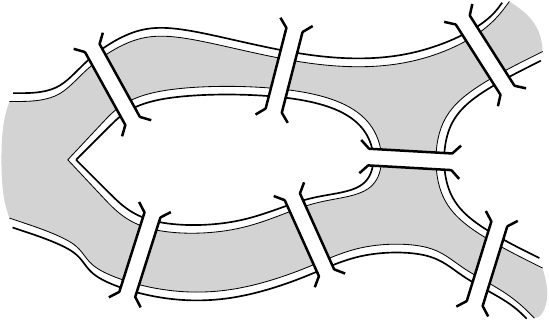
\includegraphics[width=3.5cm]{euler2.png}
\captionof{figure}{Septiņi Kēnigsbergas tilti }
\label{fig:sevenBridges}
\end{center} 
\end{problem}
%

%2
\begin{problem}
\textit{[Klasesbiedri]}
Skolnieks reiz teica Jānītim: „Mūsu klasē ir $35$ cilvēki. Un, iedomājies, katrs draudzējas  ar tieši $11$ klasesbiedriem!”
Jānītis, būdams matemātiķis, uzreiz atbildēja: „Tā būt nevar.” 
Kā viņš to varēja zināt?
\end{problem}
%

%3
\begin{problem}
\textit{[Satiksmes organizācija]}
Vakandas karaļvalstī ir $15$ pilsētas, katra no kurām ir savienota ar ne mazāk kā $7$ citām pilsētām ar ceļiem. Pierādīt, ka no katras pilsētas var nonākt jebkurā citā (iespējams, caur citām pilsētām)!
\end{problem}
%

%4
\begin{problem}
\textit{[Stieples kubs]}
Luīzei ir $120cm$ garš stieples gabals.
\begin{enumerate}
\item Vai viņa var no šīs stieples izlocīt kubu ar malas garumu $10cm$, negriežot šo stiepli?
\item Ja stiepli tomēr nepieciešams sagriezt, kāds ir mazākais nepieciešamais gabalu skaits?
\end{enumerate}
\end{problem}
%

%5
\begin{problem}
\textit{[Skriceles]}
Vai Attēlā \ref{fig:doodle} redzamo figūru ir iespējams uzzīmēt, neatraujot zīmuli no papīra?
\begin{center}
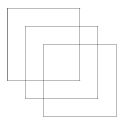
\includegraphics[width=3cm]{doodle.png}
\captionof{figure}{Skricele }
\label{fig:doodle}
\end{center} 
\end{problem}
%

%6
\begin{problem}
\textit{[Sacensību veidi]}
Sacensībās piedalās $30$ komandas. Kāds ir kopējais izspēlēto spēļu skaits, ja:
\begin{enumerate}
\item Visas komandas spēlē katra ar katru
\item Komandas spēlē play-off (katrā spēlē zaudējusī komanda izstājas, bet uzvarējusī turpina sacensības)
\end{enumerate}
\end{problem}
%

%7
\begin{problem}
\textit{[Cikliskās references]}
Uz daudzstūra malām izvietotas bultiņas. Pierādiet, ka virsotņu skaits, kurās ieiet divas bultiņas ir vienāds ar virsotņu skaitu, no kurām iziet divas bultiņas!
\end{problem}
%

%8
\begin{problem}
\textit{[Forestry]}
Par \textit{koku} sauksim tādu mezglu kopu, daži no kurām ir savienotas ar zariem (pie kam katrs zars savieno tieši divus mezglus). Kustoties pa zariem kokā, ir iespējams aiziet no jebkura mezgla uz jebkuru citu, bet nav iespējams atgriezties jau apciemotā mezglā neejot pa vienu zaru divreiz. Par \textit{lapu} kokā sauc meglu, no kura iziet tikai viens zars. 

Pierādiet, ka katrā kokā ir vismaz divas lapas!

\end{problem}
%

%9
\begin{problem}
\textit{[Tīkla stabilitāte]}
Kāds ir mazākais nepieciešamais savienojumu skaits starp $10$ informācijas pārraides mezgliem, lai garantētu to, ka, izejot no ierindas jebkuriem $2$ mezgliem, visi atlikušie mezgli joprojām būtu savienoti?
\end{problem}
%


\end{document}
